\documentclass[paper=a4, fontsize=11pt]{scrartcl} % A4 paper and 11pt font size

\newcommand{\assignment}{3}
\newcommand{\duedate}{February 15, 2023}
\usepackage[top=1in, bottom=1.5in, left=1in, right=1in]{geometry}
\usepackage{fancyhdr} % Required for custom headers
\usepackage{lastpage} % Required to determine the last page for the footer
\usepackage{extramarks} % Required for headers and footers
\usepackage[usenames,dvipsnames]{color} % Required for custom colors
\usepackage{graphicx} % Required to insert images
\usepackage{listings} % Required for insertion of code
\usepackage{courier} % Required for the courier font
\usepackage{amsmath}
\usepackage[super]{nth}
\usepackage{booktabs}
\usepackage[usenames,dvipsnames]{xcolor}
\usepackage{tcolorbox}
\usepackage{tabularx}
\usepackage{array}
\usepackage{colortbl}

%\usepackage[T1]{fontenc} % Use 8-bit encoding that has 256 glyphs
%\usepackage{fourier} % Use the Adobe Utopia font for the document - comment this line to return to the LaTeX default
\usepackage[english]{babel} % English language/hyphenation
\usepackage{amsmath,amsfonts,amsthm} % Math packages
\usepackage{graphicx}

\usepackage{hyperref}
\hypersetup{
  colorlinks   = true, %Colours links instead of ugly boxes
  urlcolor     = blue, %Colour for external hyperlinks
  linkcolor    = blue, %Colour of internal links
  citecolor   = red %Colour of citations
}

\usepackage{fancyhdr} % Custom headers and footers
\pagestyle{fancyplain} % Makes all pages in the document conform to the custom headers and footers
\fancyhead{} % No page header - if you want one, create it in the same way as the footers below
\fancyfoot[L]{} % Empty left footer
\fancyfoot[C]{} % Empty center footer
\fancyfoot[R]{\thepage} % Page numbering for right footer
\renewcommand{\headrulewidth}{0pt} % Remove header underlines
\renewcommand{\footrulewidth}{0pt} % Remove footer underlines
\setlength{\headheight}{13.6pt} % Customize the height of the header
\newcommand{\ts}{\textsuperscript}

\numberwithin{equation}{section} % Number equations within sections (i.e. 1.1, 1.2, 2.1, 2.2 instead of 1, 2, 3, 4)
\numberwithin{figure}{section} % Number figures within sections (i.e. 1.1, 1.2, 2.1, 2.2 instead of 1, 2, 3, 4)
\numberwithin{table}{section} % Number tables within sections (i.e. 1.1, 1.2, 2.1, 2.2 instead of 1, 2, 3, 4)

\setlength\parindent{0pt} % Removes all indentation from paragraphs - comment this line for an assignment with lots of text

% Default fixed font does not support bold face
\DeclareFixedFont{\ttb}{T1}{txtt}{bx}{n}{8} % for bold
\DeclareFixedFont{\ttm}{T1}{txtt}{m}{n}{8}  % for normal

%----------------------------------------------------------------------------------------
%	CODE BLOCKS
%----------------------------------------------------------------------------------------

\usepackage{adjustbox}
\usepackage{listings}
\usepackage{color}

\definecolor{dkgreen}{rgb}{0,0.6,0}
\definecolor{gray}{rgb}{0.5,0.5,0.5}
\definecolor{mauve}{rgb}{0.58,0,0.82}

\lstdefinelanguage{Dockerfile}
{
  morekeywords={FROM, RUN, CMD, LABEL, MAINTAINER, EXPOSE, ENV, ADD, COPY,
    ENTRYPOINT, VOLUME, USER, WORKDIR, ARG, ONBUILD, STOPSIGNAL, HEALTHCHECK,
    SHELL},
  morecomment=[l]{\#},
  morestring=[b]"
}

\lstset{
    columns=flexible,
    aboveskip=5mm,
    belowskip=5mm,
    keepspaces=true,
    showstringspaces=false,
    basicstyle=\ttfamily,
    commentstyle=\color{gray},
    keywordstyle=\color{purple},
    stringstyle=\color{green}
}



%----------------------------------------------------------------------------------------
%	TITLE SECTION
%----------------------------------------------------------------------------------------

\usepackage{eso-pic}
% \usepackage[demo]{graphicx}
\newcommand\AtPageUpperRight[1]{\AtPageUpperLeft{%
   \makebox[\paperwidth][r]{#1}}}

\newcommand{\horrule}[1]{\rule{\linewidth}{#1}} % Create horizontal rule command with 1 argument of height

\title{	
\normalfont \normalsize
\textsc{Northeastern University,  Khoury College of Computer Science} \\ [25pt] % Your university, school and/or department name(s)
\horrule{0.5pt} \\[0.4cm] % Thin top horizontal rule
\huge CS 6220  Data Mining \textemdash~Assignment \assignment \\ % The assignment title
\Large \textbf{Due: \duedate (100 points)} % The assignment title
\horrule{2pt} \\[0.5cm] % Thick bottom horizontal rule
}

% Original in the document
\AddToShipoutPictureBG*{%
  \AtPageUpperRight{\raisebox{-\height}{
\includegraphics[width=3cm]{images/logo}}}}

\author{
    \textbf{YOUR NAME} \\ 
    \textbf{YOUR GIT USERNAME} \\ 
    \textbf{YOUR E-MAIL}
}% INFORMATION

\date{} % Today's date or a custom date
\author{
    \textbf{YOUR NAME} \\ 
    \textbf{YOUR GIT USERNAME} \\ 
    \textbf{YOUR E-MAIL}
}% INFORMATION

\begin{document}

\maketitle % Print the title

\vspace{5mm}
{\Large \textbf{Question 1} [50 pts]} \\

Preprocess the the data with \textbf{z-score normalization} and scatter the data that's been projected onto the first two principle components with different colors for each target/class of wine. Include your code (linked or inline).\\
\begin{verbatim}
import numpy as np
from sklearn.datasets import load_wine
from sklearn.preprocessing import StandardScaler
from sklearn.decomposition import PCA
import matplotlib.pyplot as plt

wine = load_wine()
x = wine.data
y = wine.target
scale = StandardScaler()
x_normalized = scale.fit_transform(x)
pca = PCA(n_components=2)
pca.fit(x)
x_pca = pca.transform(x)
ratio = pca.explained_variance_ratio_

for item in np.unique(y):
    idx = (y==item)
    plt.scatter(x_pca[idx,0],x_pca[idx,1],label=f'class_{item}')

plt.title('PCA with Raw wine data')
plt.xlabel(f'PC1: {np.round(100*ratio[0],4)}%')
plt.ylabel(f'PC2: {np.round(100*ratio[1],4)}%')
plt.legend()
plt.show()
\end{verbatim} \\


\begin{center}
    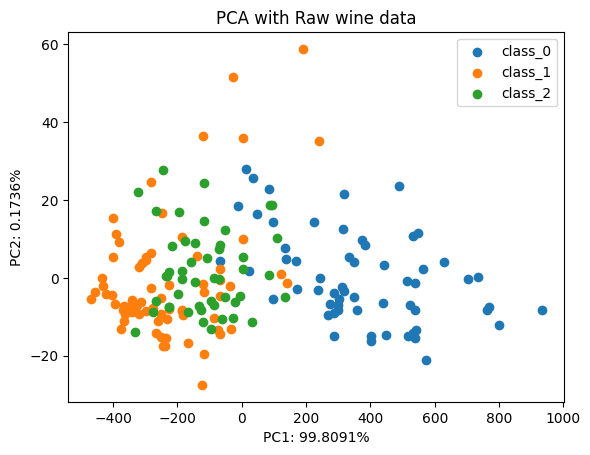
\includegraphics[width=75mm]{images/pca.png}
\end{center}

{\huge \textbf{Parameter Estimation}} \\

It is well-known that light bulbs commonly go out according to a Poisson distribution, and are independent regardless of whether or not they're made in the same factory. The Poisson distribution has the form: \\
\begin{equation}
p(X | \lambda) = \frac{ \exp^{-\lambda} \lambda ^{x_i}}{ x_i !} \nonumber
\end{equation} \\

An architect has outfitted a building with 32,000 of the same lightbulb. The factory has provided him with data on when $N$ of these lightbulbs have gone out over their lifetimes. They've been measured with $\mathcal{D} = \{ x_1, x_2, \cdots, x_N \}$\\
\\
{\Large \textbf{Question 2} [50 pts]} \\
\\
Derive the maximum likelihood estimate of the parameter $\lambda$ in terms of $x_i$. Please show your work. \\
\\
$$
\begin{aligned}
f(\mathcal{D}) &= \prod_{i=1}^{N}p(x_i|\lambda) \\
&= \prod_{i=1}^{N}\frac{e^{-\lambda}\lambda^{x_i}}{x_i!} \\
\end{aligned}
$$

Maximize $f(\mathcal{D})$ is equivalent to maximizing $\log f(\mathcal{D})$.
$$
\begin{aligned}
\log f(\mathcal{D}) &= \sum_{i=1}^{N}\log p(x_i|\lambda) \\
&= \sum_{i=1}^{N}\left( -\lambda + x_i\log\lambda -\log(x_i!) \right) \\
&= -N\lambda + (\log\lambda)\sum_{i=1}^{N}x_i - \sum_{i=1}^{N}\log(x_i!) \\
\end{aligned}
$$

Then we obtain derivative of $\log f(\mathcal{D})$ as:
$$
\frac{\partial \log f(\mathcal{D})}{\partial \lambda} = -N + \frac{\sum_{i=1}^{N}x_i}{\lambda}
$$

Let the derivative to be 0. We can obtain the estimated value of parameter $\lambda$.
$$
\lambda^\ast = \frac{\sum_{i=1}^{N}x_i}{N}
$$

%%%%%%%%%%%%%%%%%%%%


\end{document}
